\documentclass[11pt]{article}
\usepackage[a4paper, margin=2.5cm]{geometry}

\usepackage[utf8]{inputenc}
\usepackage[T1]{fontenc}
\usepackage[slovene]{babel}

\usepackage{graphicx}

\title{Brownovo gibanje}
\author{Matej Rojec}
\date{}

\usepackage{amsthm}
\theoremstyle{definition}
\newtheorem{definicija}{Definicija}

\theoremstyle{plain}
\newtheorem{izrek}{Izrek}

\begin{document}

Brownovo gibanje (več v ??) je intuitivno slučajen proces, % Sklic na knjigo
ki predstavlja naključno gibanje delcev v mediju.
\begin{figure}[htbp]
  \centering
  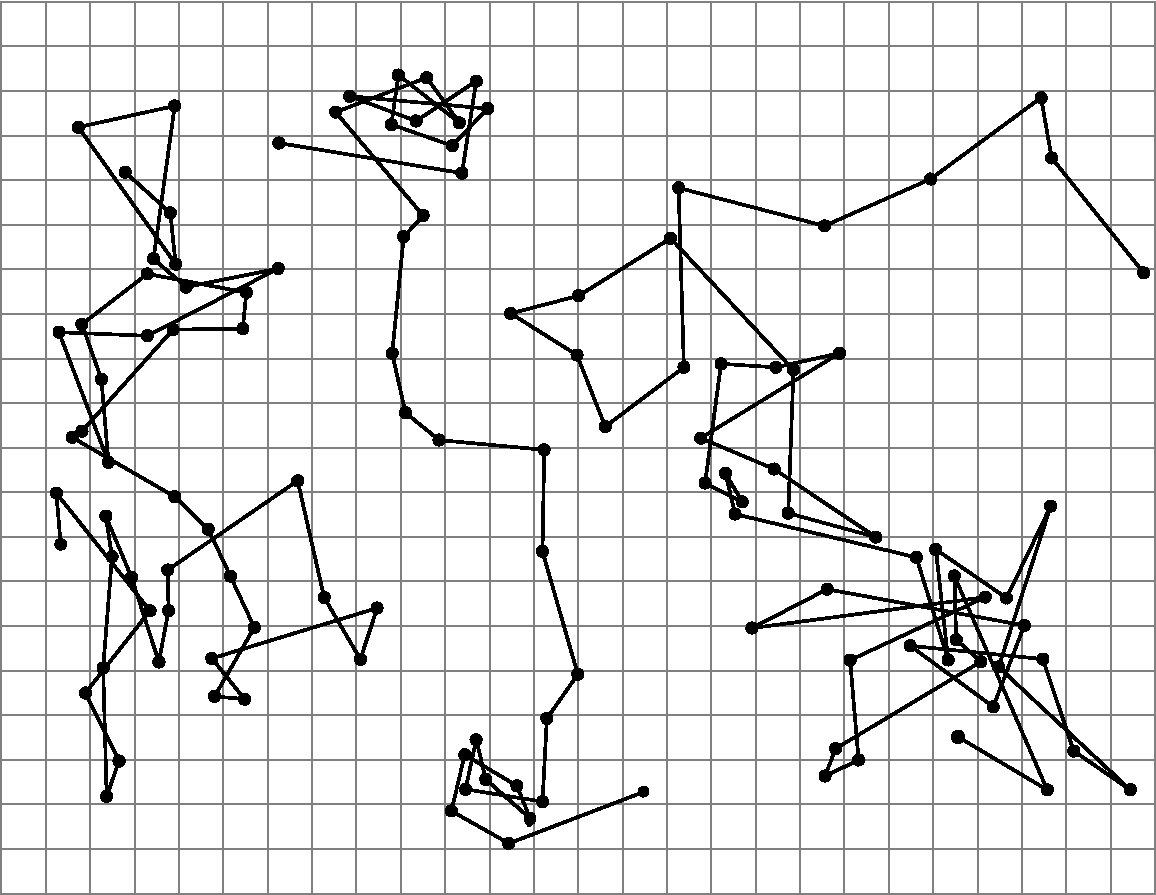
\includegraphics[width=0.3\textwidth]{PerrinPlot2.pdf}  
  \caption{Reprodukcija slike iz Jean Baptiste Perrin}
  \label{fig:brownovo-gibanje}
\end{figure}   
    % Slika: PerrinPlot2.pdf, velikost scale=0.3
    % Napis pod sliko: 
    % Reprodukcija slike iz Jean Baptiste Perrin, \emph{Mouvement brownien et réalité moléculaire}, Ann. de Chimie et de Physique (VIII) 18, 5-114, 1909

    % Začetek definicije
    \begin{definicija}
    Standardno Brownovo gibanje \(\{B_t\}_{t \geq 0}\) je slučajen proces z naslednjimi lastnostmi: 
    \begin{itemize}
        \item\(B_0 = 0\).
        \item Prirastki \(B_{t_n} - B_{t_{n-1}}, B_{t_{n-1}} - B_{t_{n-2}}, \ldots, B_{t_2} - B_{t_1}, B_{t_1} - B_{t_0}\) so neodvisne slučajne spremenljivke, za vsak \(t_0 \leq t_1 \leq \cdots \leq t_{n-1} \leq t_n\).
        \item Za vsak \(t \geq 0\) in \(h > 0\) velja \(B_{t+h} - B_t \sim \mathcal{N}(0, h)\).
        \item Funkcija \(t \mapsto B_t\) je zvezna skoraj gotovo.
        \end{itemize}
    \end{definicija}
    % Konec definicije
    
    Preden zapišemo izrek, definirajmo še pojem časa ustavljanja.
    
    % Začetek definicije
    \begin{definicija}
    Slučajna spremenljivka \(\tau\) na verjetnostnem prostoru !! z vrednostmi v !!
    je čas ustavljanja glede na filtracijo !!, če velja: !!.
    \end{definicija}
    % Konec definicije
    
    Zdaj lahko zapišemo izrek ??. % Sklic na izrek z oznako thm:stopped_brownian
    
    % Začetek izreka
    \begin{izrek}
    Naj bo \(\{B_t\}_{t \geq 0}\) (standardno) Brownovo gibanje, \(\tau\) čas ustavljanja glede na
    !! in naj velja !!.
    Potem je tudi proces:
    \[
    \hat{B} := \{B_{\tau+t} - B_\tau \mid t \geq 0\}
    \]
    (standardno) Brownovo gibanje in neodvisen od !!.
    \end{izrek}
    % Konec izreka
    
\end{document}